\documentclass[11pt,a4paper]{article}
\usepackage{babel}
\usepackage{array}
\usepackage{tabularx}
\usepackage{fancyhdr}
\usepackage{fancyvrb}
\usepackage{multicol}
\usepackage{listings}
\usepackage{graphicx}
\graphicspath{{I:\\##VISHESH##\\pp python project }}
\usepackage[hmargin=1.5cm,
vmargin=1.5cm]{geometry}


\usepackage[dvipsnames]{xcolor}

\usepackage{fancyvrb}









\begin{document}
\pagestyle{fancy}
\lhead{Vishesh Chouhan}
\rhead{0801CS211101}
\fancyfoot{}
\fancyfoot[R]{{\small\thepage}}
\renewcommand{\footrulewidth}{0.4pt}


\begin{flushleft}
	\textbf{\Large Objectives of project}\\
	To create a program that produces the bill of the plants that are sold by the seller in a user friendly graphical interface.\\


	\textbf{\Large \\ Function description}
	
	\begin{itemize}
	
	
	\item \textbf{buyrose} Initiate a dialog box to enter the quantity of rose that seller selects and add the rose into the bill with its respective quantity\\
	\item \textbf{buysunflower} Generate a dialog box that accepts the quantity of sunflower that seller selects and add the sunflower plant into the bill with its respective quantity\\
	\item \textbf{buyjasmine} Pops a selection box to enter the number of jasmine plant that seller selects and add the jasmine plant into the bill with its respective quantity\\
	\item \textbf{buyaloevera} Generate a dialog box that accepts the number of aloevera that seller selects and add the aloevera plant into the bill with its respective quantity.
	\item \textbf{buymoneyplant} Opens a selection box to take the amount of moneyplant that seller selects and add the moneyplant into the bill with its respective quantity\\
	\item \textbf{buyjade} Initiate a dialog box to enter the quantity of jade that seller selects and add the jade into the bill with its respective quantity\\
	
	\item \textbf{buyadenium} Generate a dialog box that accepts the quantity of adenium plant that seller selects and add the sunflower plant into the bill with its respective quantity\\
	\item \textbf{buycactus} Pops a selection box to enter the number of cactus plant that seller selects and add the cactus plant into the bill with its respective quantity\\
	\item \textbf{buypalm} Initiate a dialog box to enter the quantity of palm that seller selects and add the palm into the bill with its respective quantity\\
	
	\item \textbf{gotoflower} Open up another window that contains different varieties of plant in the same domain. It will open up the flower category\\
	
	\item \textbf{gotodecoration}This function open up another window that contains different varieties of plant in the same domain. It will open up the category of plant that are usually used for decoration\\
	
	\item \textbf{gotodesert} The plants that belong to the desert are selected by this function. It will pop up a window that contains desert plants.\\
	
	\item \textbf{billf} Generates the bill of the plants that are sold with the respective quantity, and the total amount corresponding to various plants.
	It also gives the total amount the buyer has to pay\\
	
	\item \textbf{billf} Sort the bill in aplhabetic manner with respect to the plants name.\\
	
	\item \textbf{change...} Change the quantity of the plants to include in the bill. change... indicates function starts with change \\
	
	\item \textbf{...price\_change} Change the price of the plants to include in the bill. ...price\_chane indicates function that changes the price of plants. \\
	
	\item \textbf{sort\_list} Sorts the list into ascending order. \\
	
	\item \textbf{print\_bill} Generates the pdf of the required invoice. \\
	
	
	\item \textbf{main} It is the runner of the code. It initializes the program.\\
	\end{itemize}
	
\end{flushleft}
\pagebreak


\begin{center}
	\textbf{PROGRAM CODE}
\end{center}


        

\vspace{.5cm}

\lstinputlisting[language=Python]{bill_generator_with_changes.py}

\pagebreak

\begin{center}
	\textbf{\Large PROGRAM OUTPUT}
\end{center}

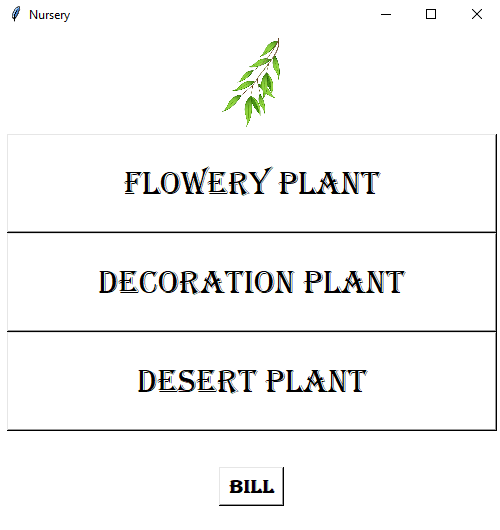
\includegraphics{output1.png}\\
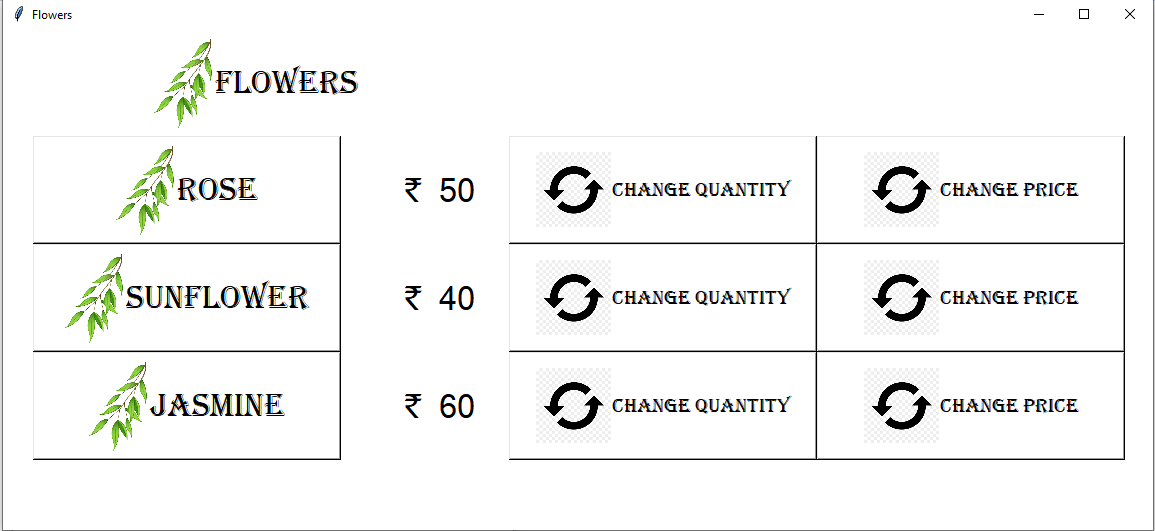
\includegraphics[scale = .6]{output2.png}\\
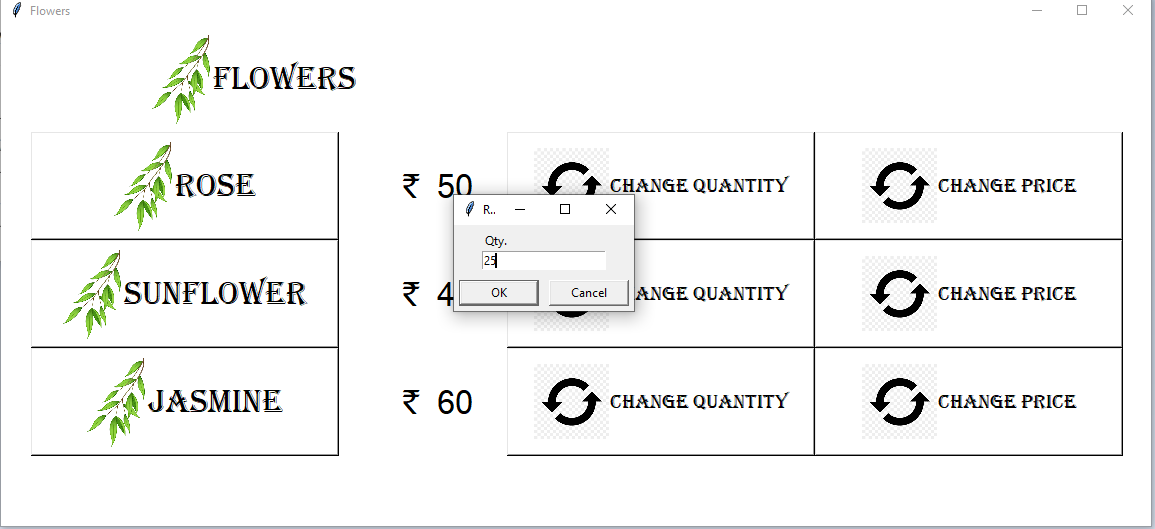
\includegraphics[scale = .6]{output3.png}\\
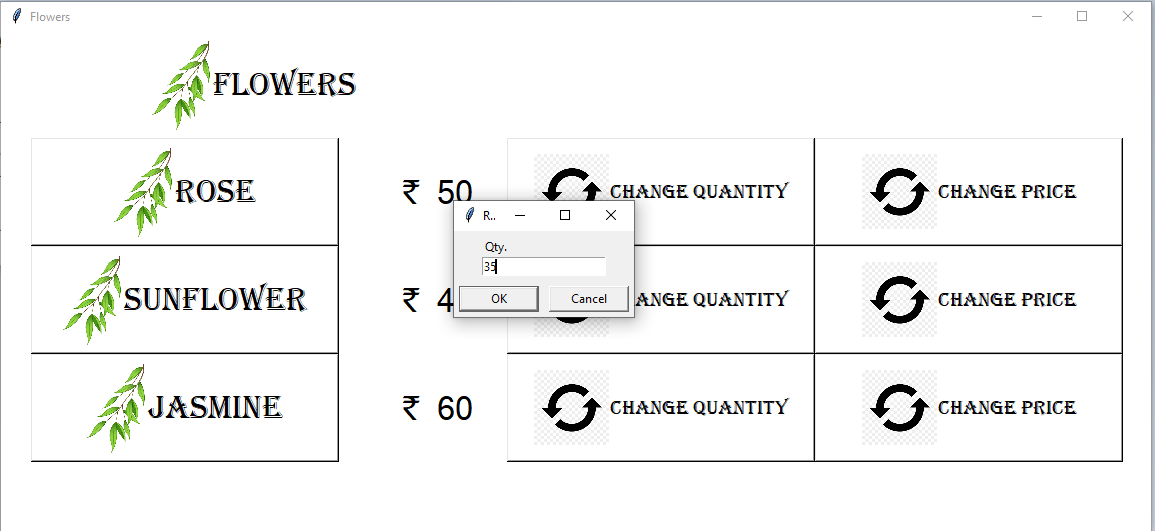
\includegraphics[scale = .6]{output4.png}\\
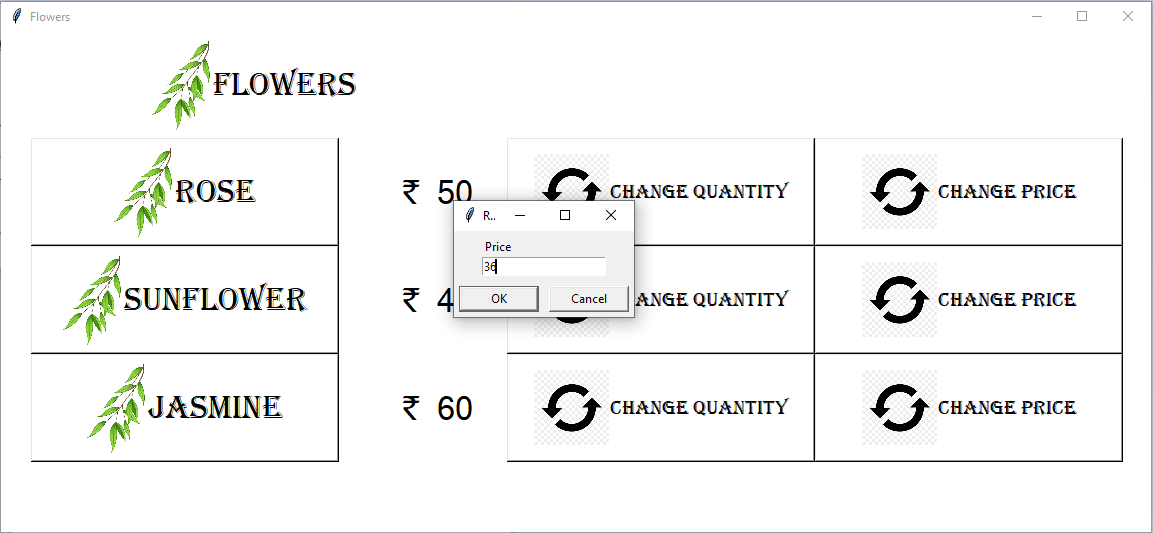
\includegraphics[scale = .6]{output5.png}\\
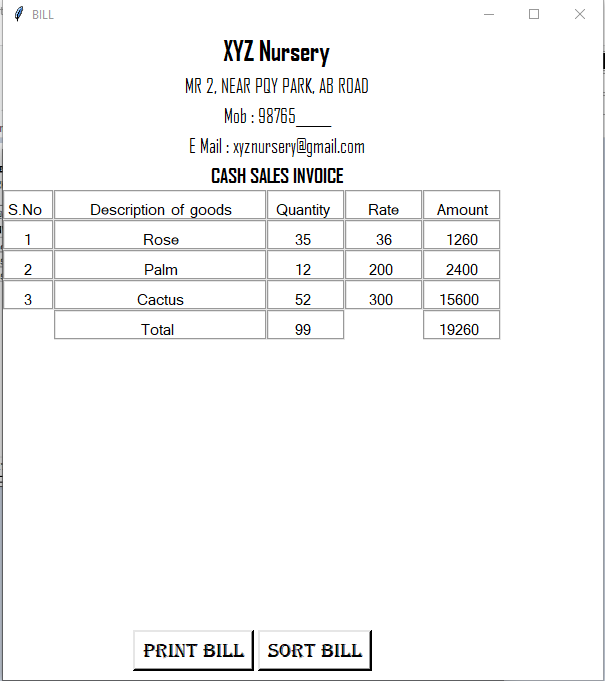
\includegraphics{output6.png}\\
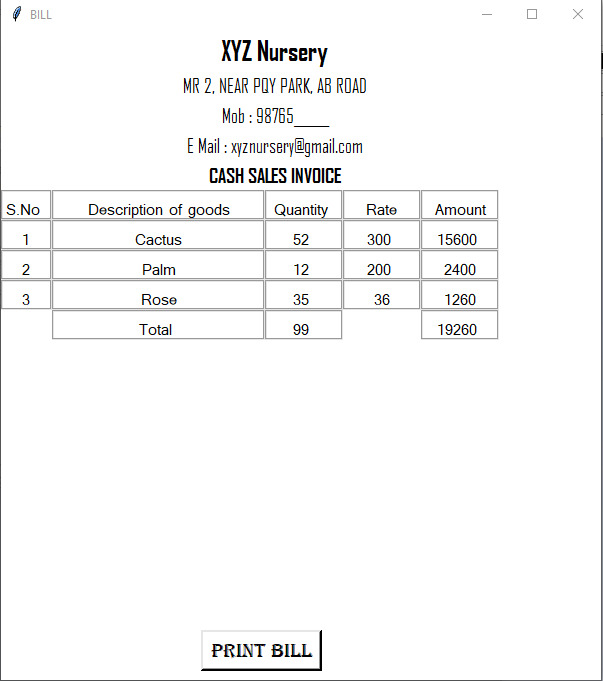
\includegraphics{output7.png}\\
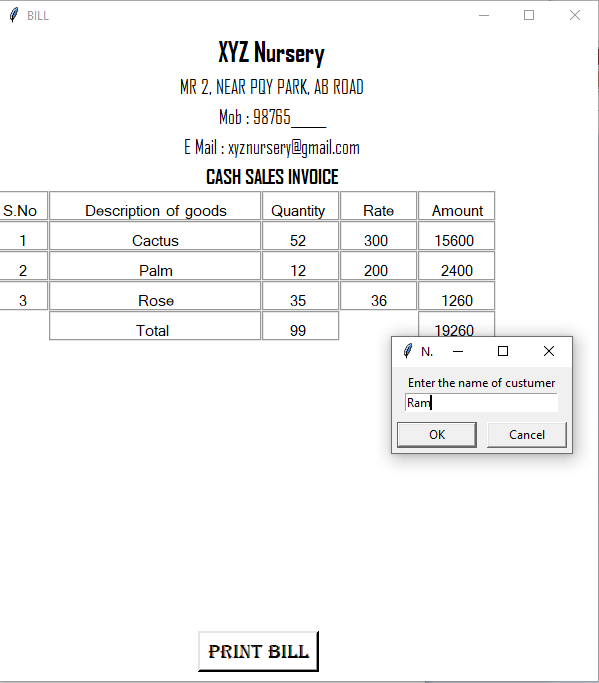
\includegraphics{output8.png}\\
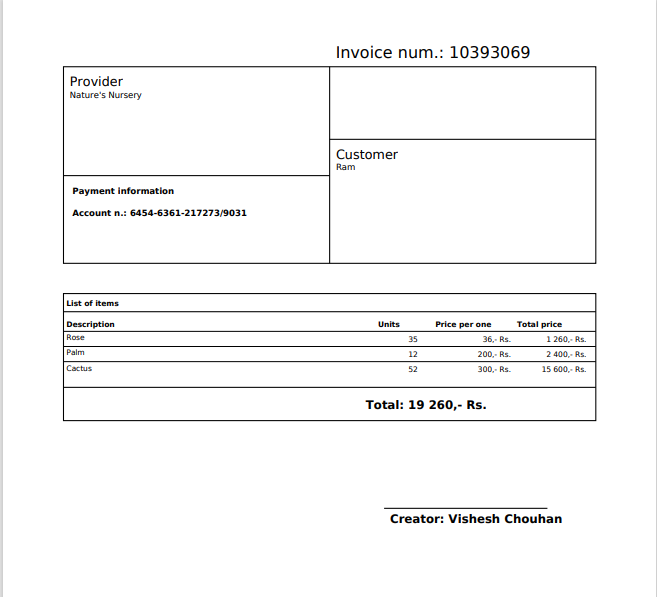
\includegraphics{output9.png}\\


\pagebreak

\begin{center}
\textbf{PROFILLING DATA}\\
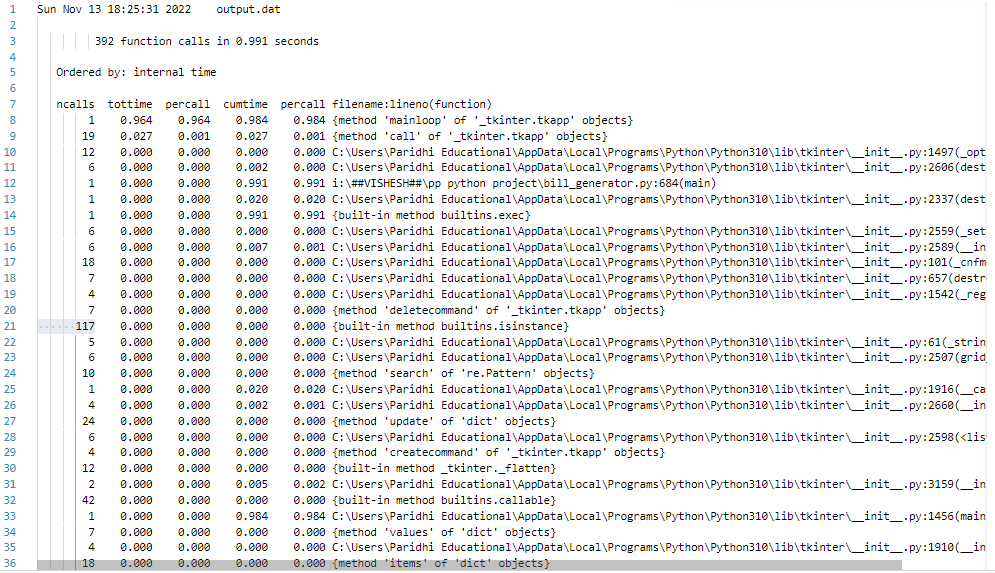
\includegraphics[scale = .7]{profiling1.png}\\
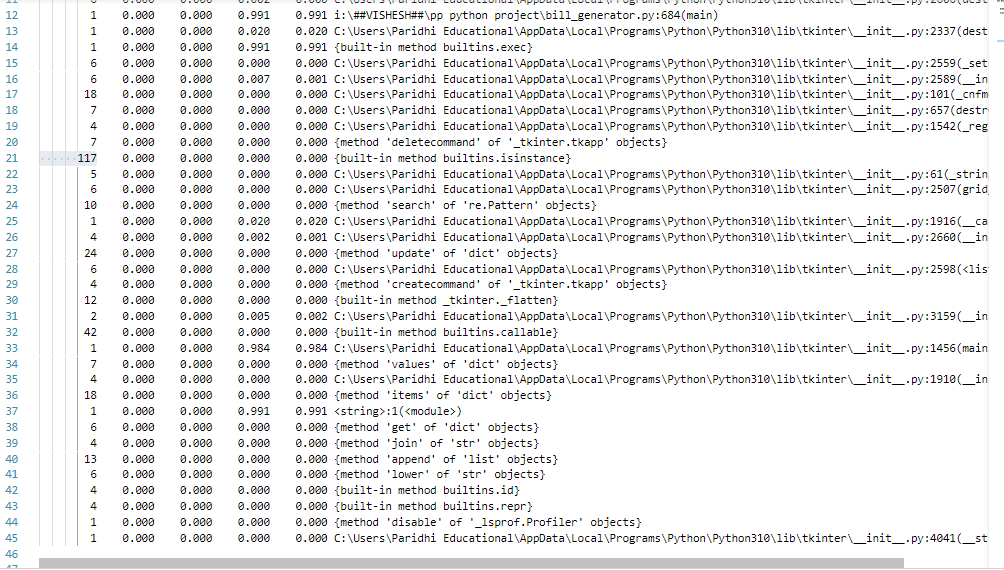
\includegraphics[scale = .7]{profiling2.png}\\
\end{center}


\pagebreak

\begin{center}
\textbf{DEBBUGING STEPS}\\
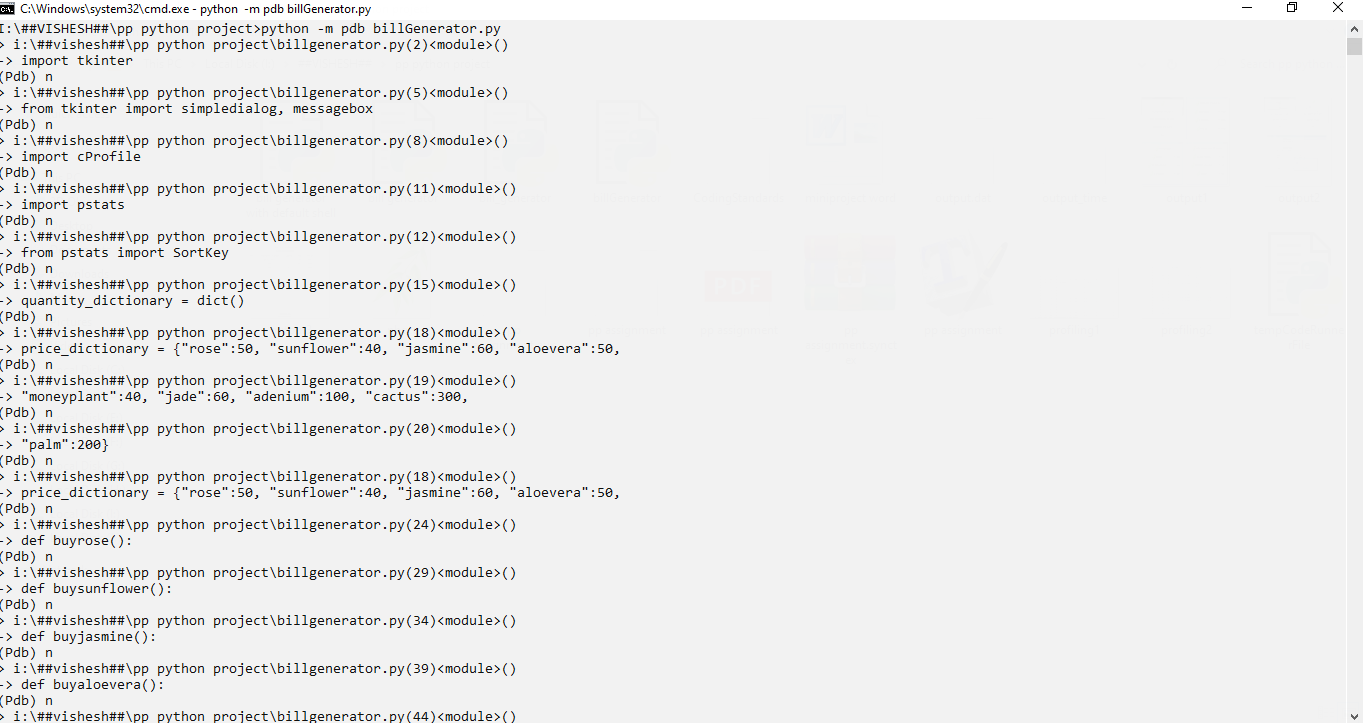
\includegraphics{debug1.png}\\
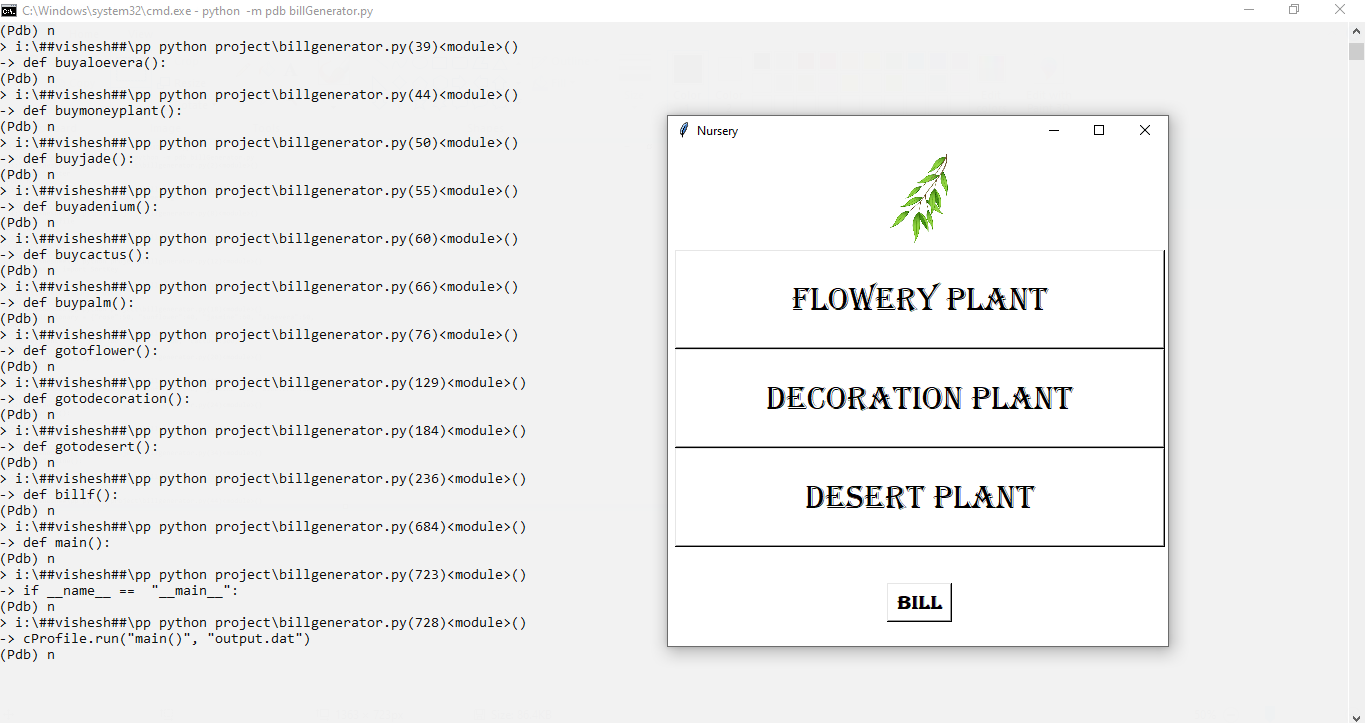
\includegraphics[scale = .6]{debug2.png}\\
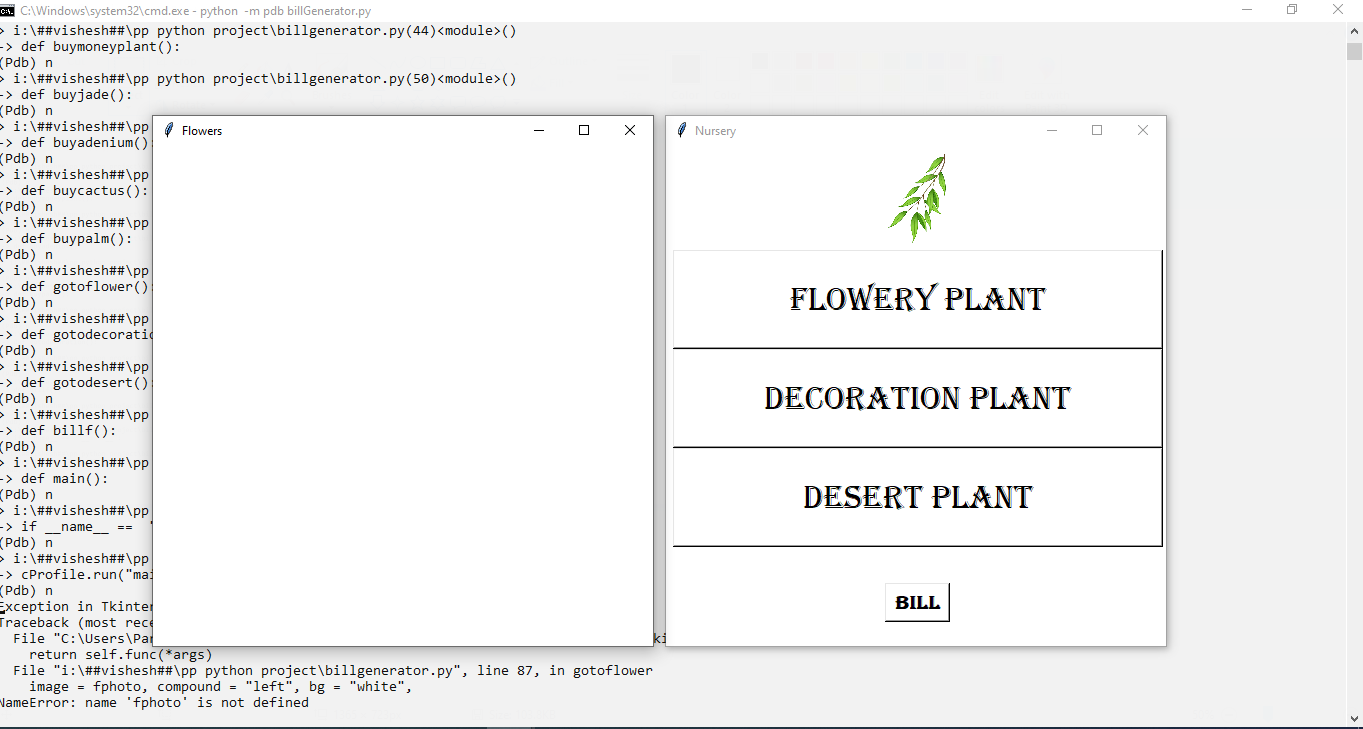
\includegraphics[scale = .6]{debug3.png}\\
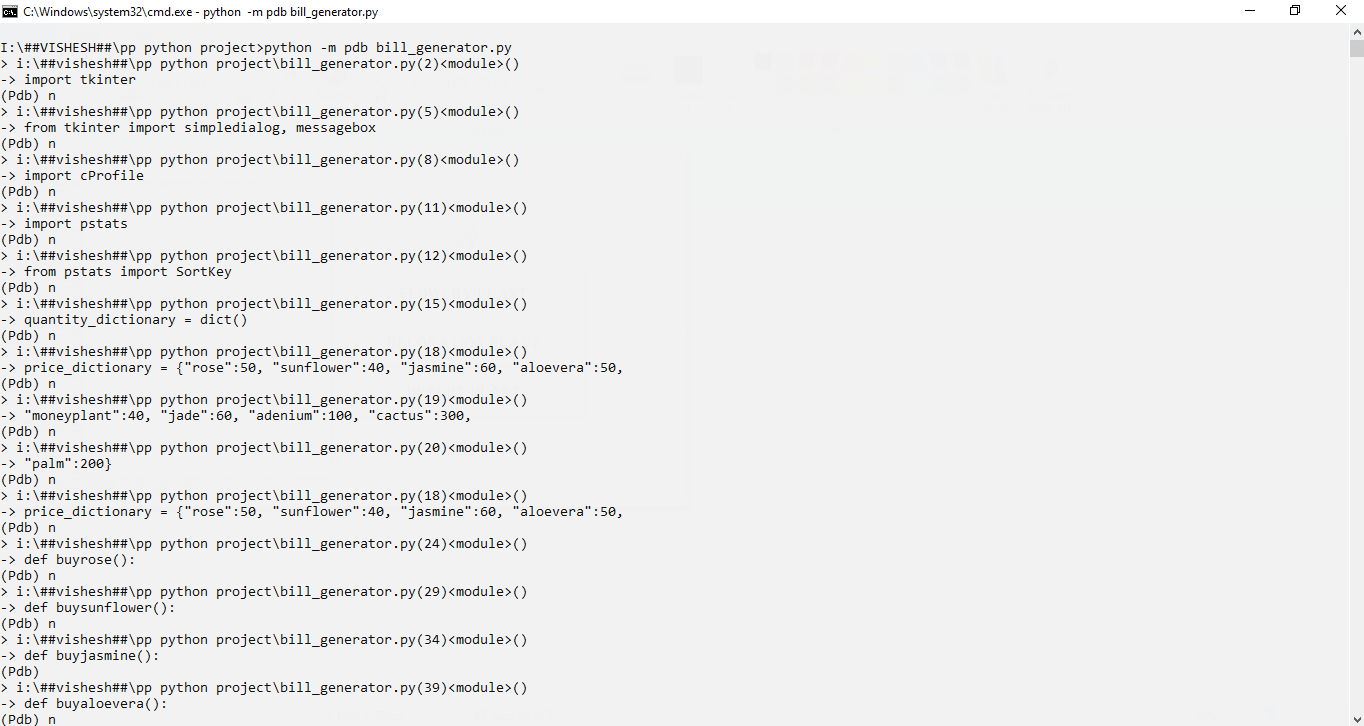
\includegraphics{debug4.png}\\
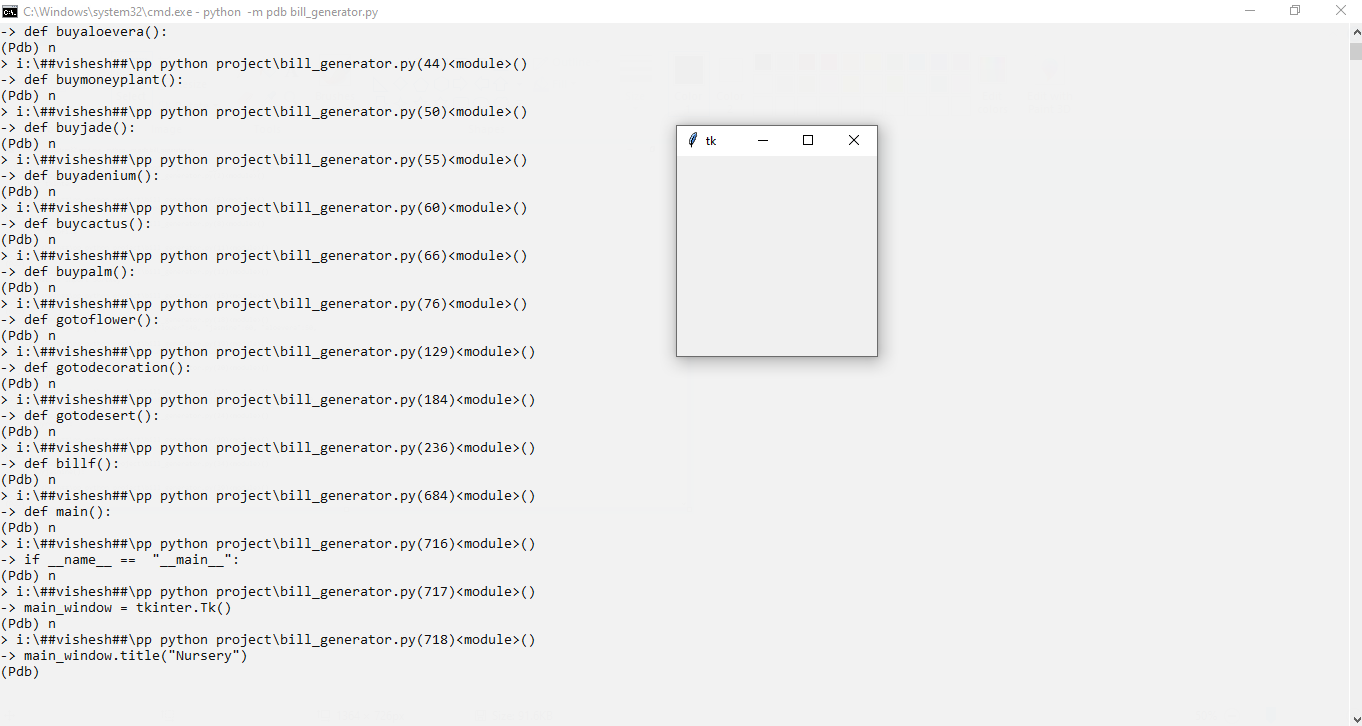
\includegraphics[scale = .6]{debug5.png}\\
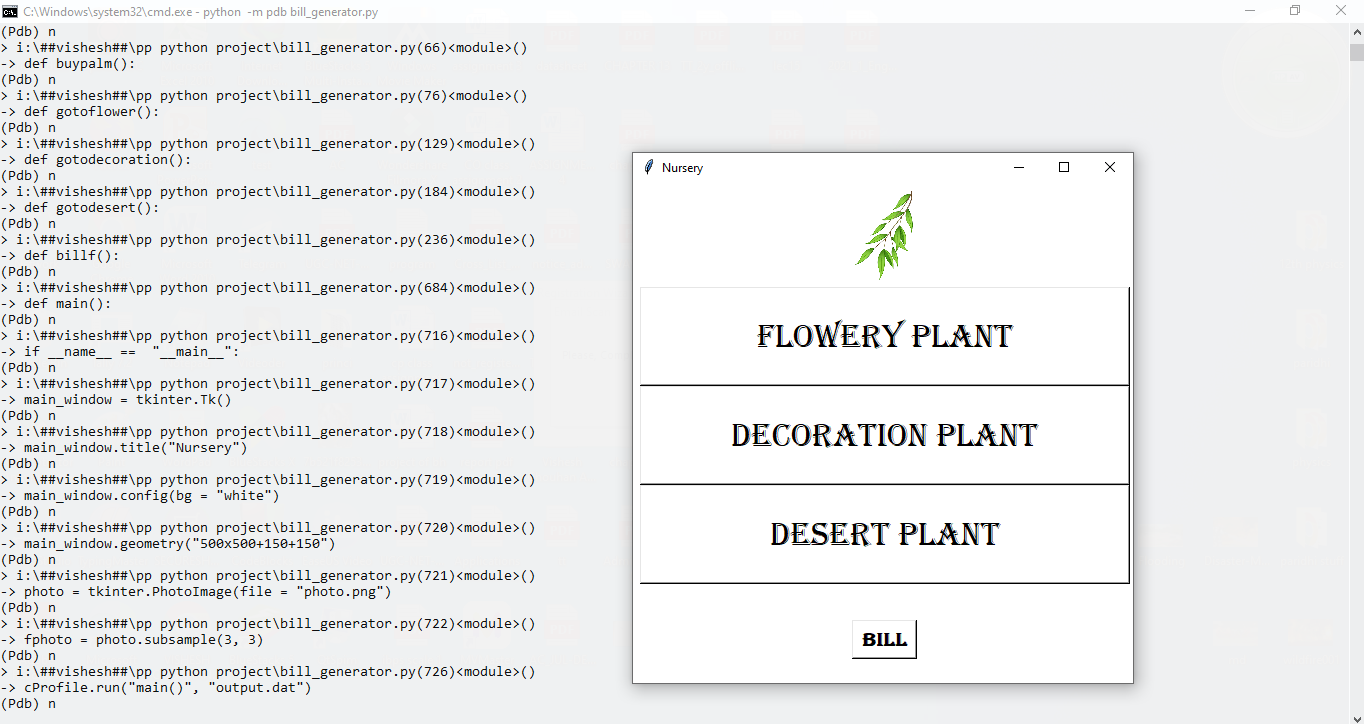
\includegraphics[scale = .6]{debug6.png}\\
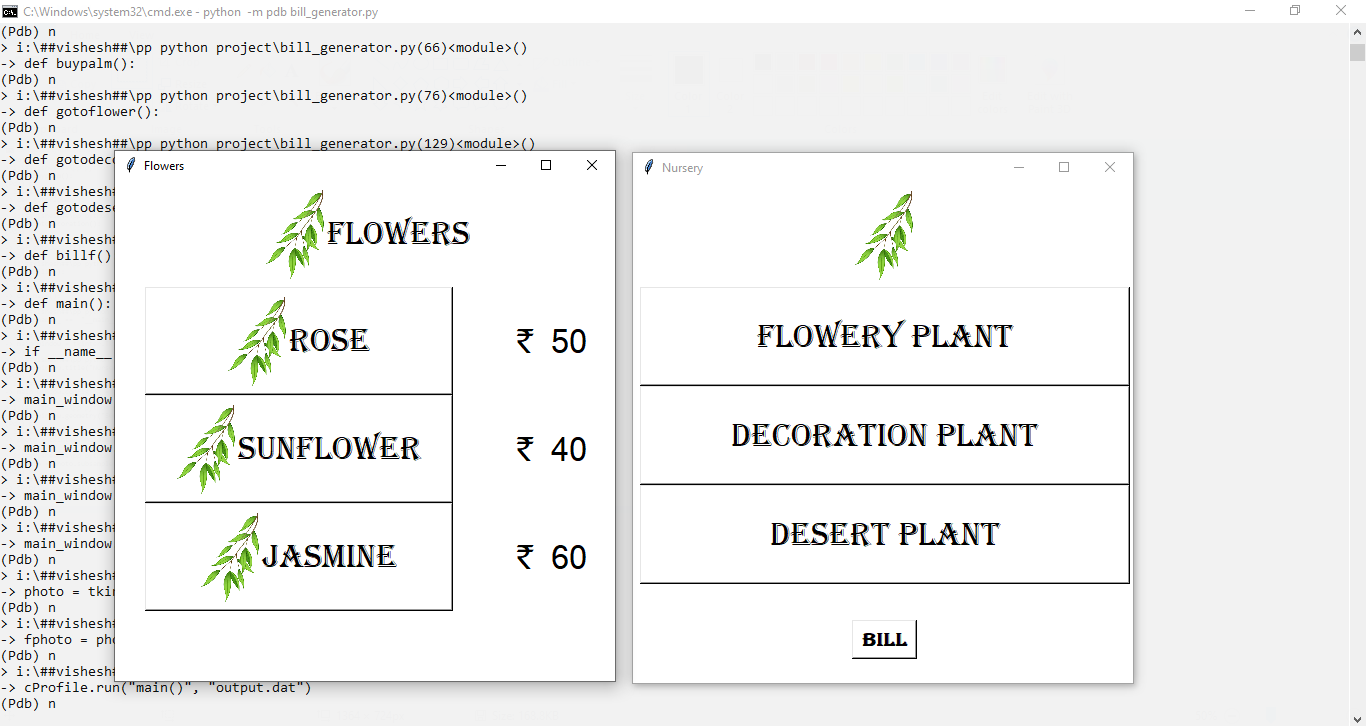
\includegraphics[scale = .6]{debug7.png}\\

\end{center}


\pagebreak

\begin{center}
	\textbf{MISCELLANEOUS DATA}
\end{center}

\begin{flushleft}
Starting Date : 5 November, 2022 \\
End Date : 13 November, 2022\\
Total time required : 9 Days\\
Total line of code : 733\\
No of functions : 15\\
Language used : Python\\
Profiller used : cProfile\\
Debugger used : pdb\\
Program Title : Bill Generator\\

\end{flushleft}
\end{document}



























